\section{Results}
\label{sec:results}

Using the $Beta\_SSE$ score with $T=36$, we construct a time series of the level of market efficiency as 
seen in Figure~\ref{fig:sp_500_SSE_beta_ts}.
\begin{figure}[h!]
    \centering
    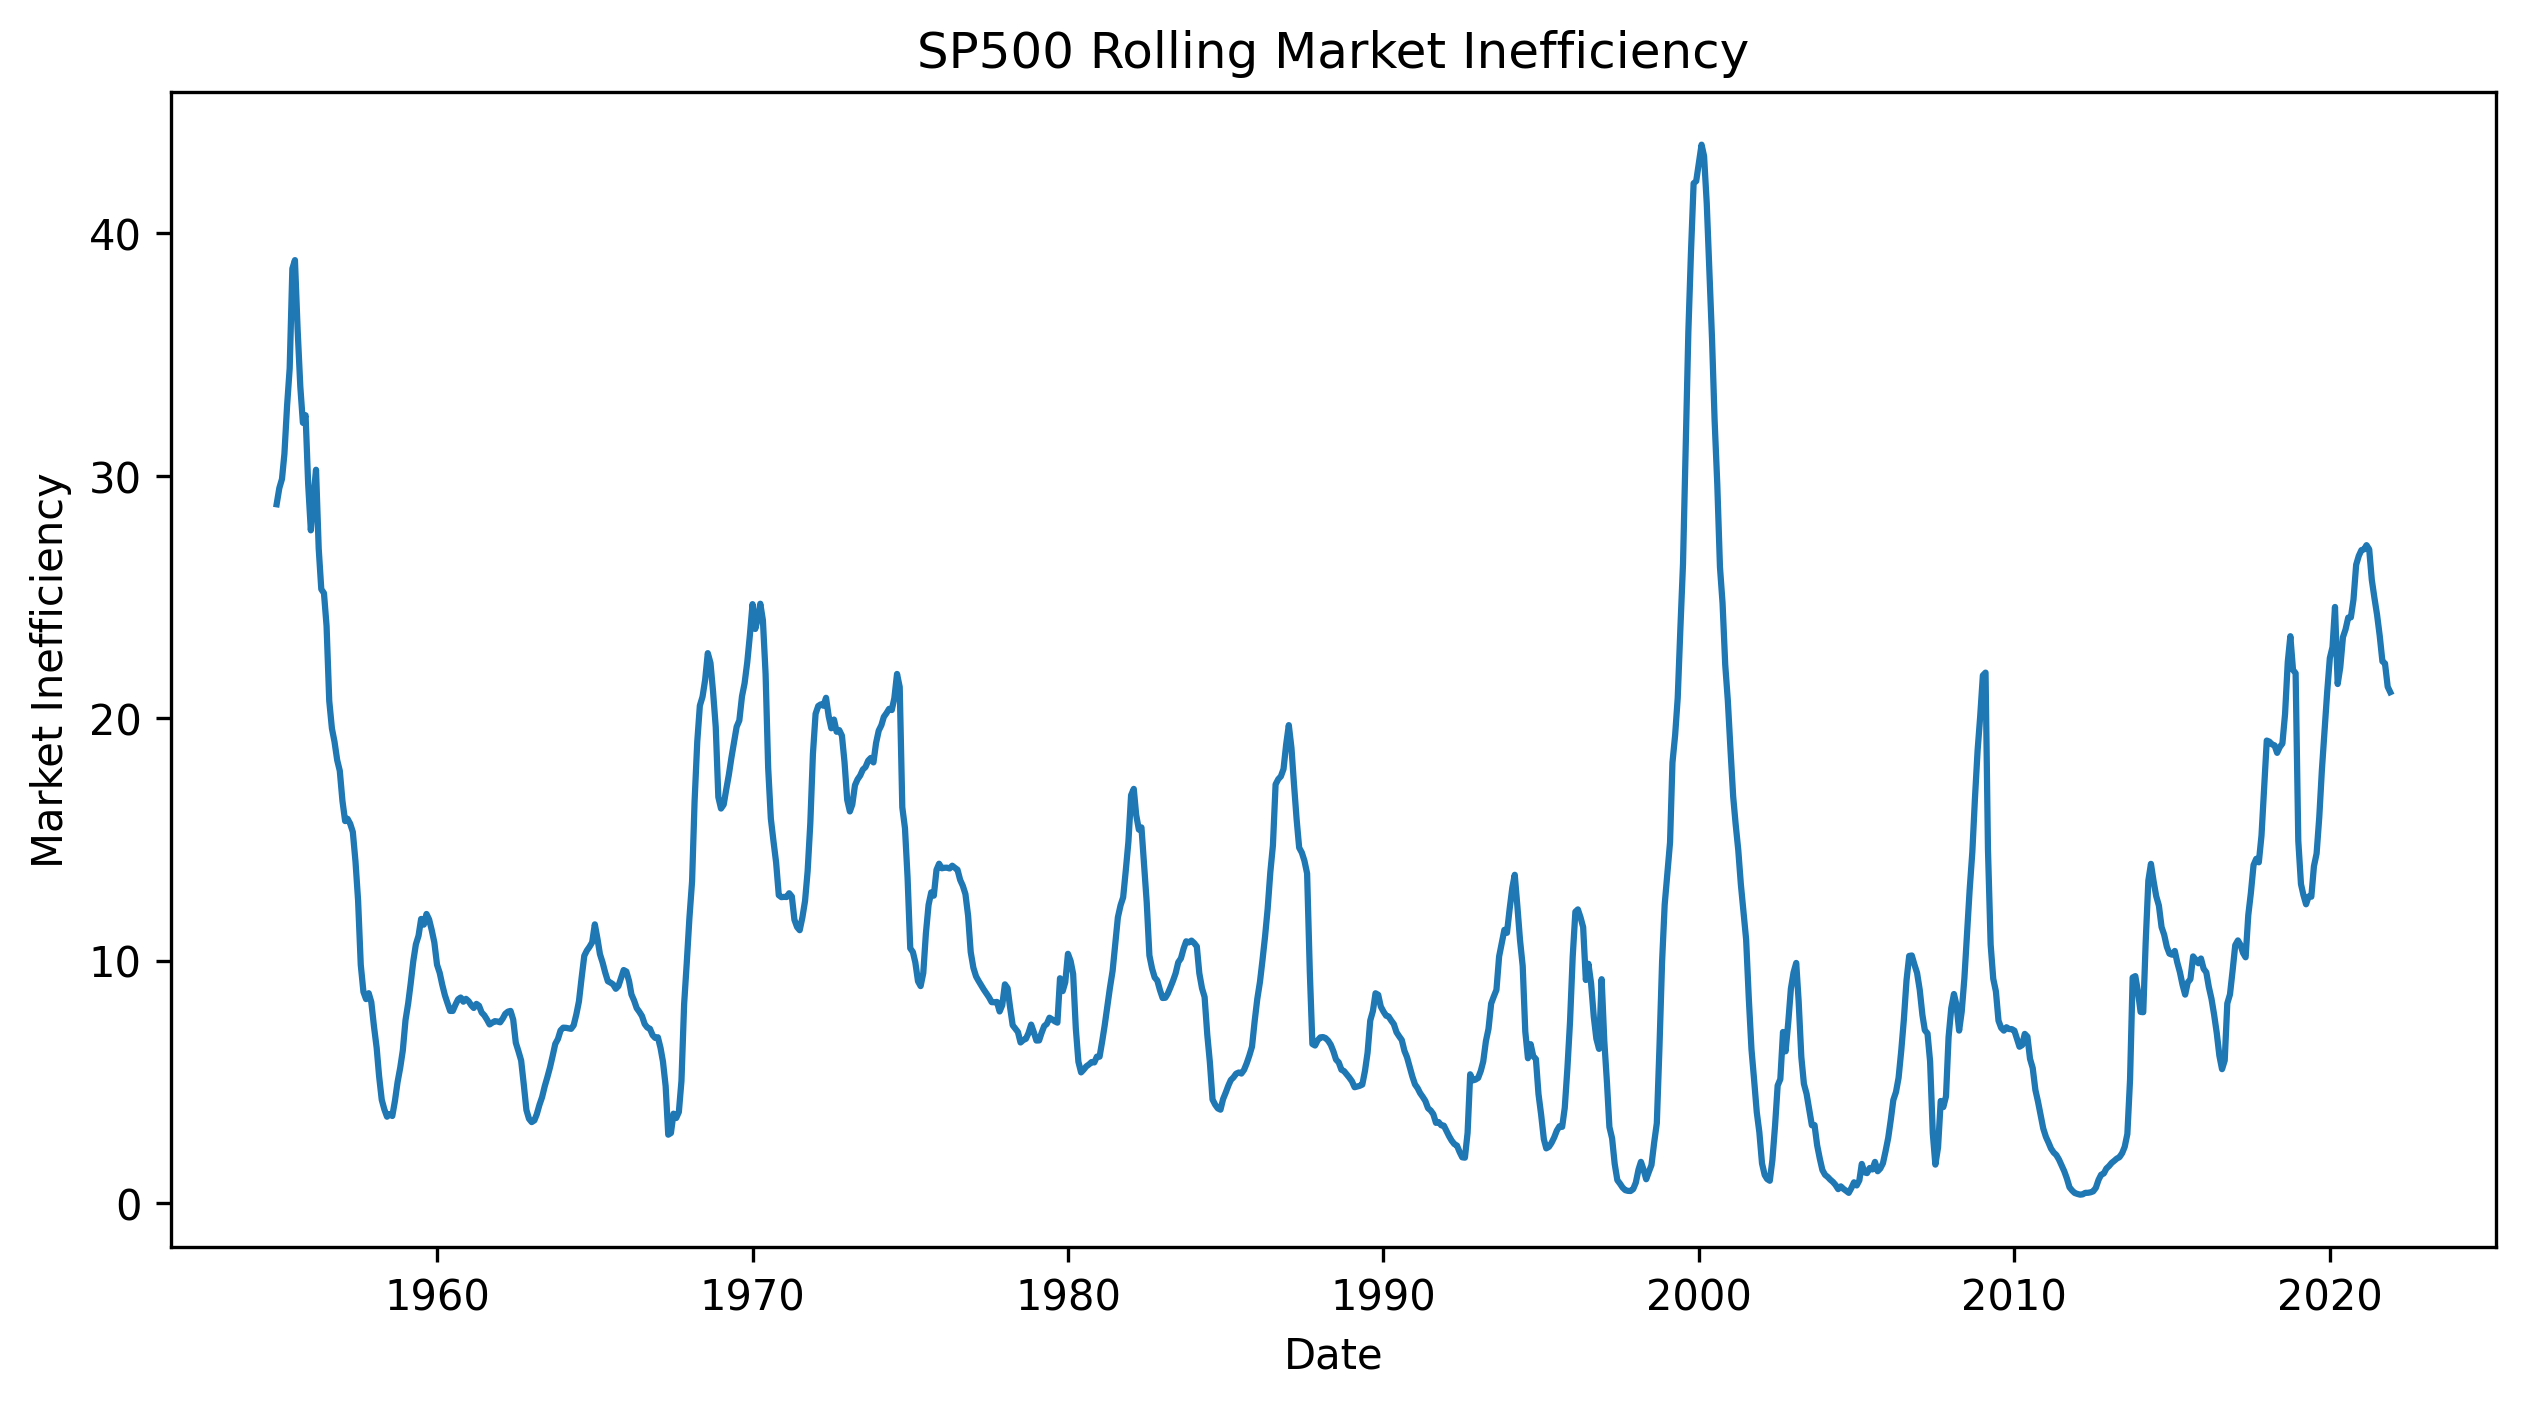
\includegraphics[width=1\textwidth]{../figs/SP500_Rolling_Market_Inefficiency.png}
    \caption{The $Beta\_SSE$ score time series of the SP500 (1950 - 2024) showing mean reversion and periods of inefficiency.}
    \label{fig:sp_500_SSE_beta_ts}
\end{figure}

We see the market is inefficient around the dot-com bubble, the 2008 financial crisis, and the COVID-19 pandemic, which is in line with our expectations.
These are times the market had to contend with inefficient pricing due to uncertainty and information asymmetry.
We can visually assess that the market is not uniformly efficient. Instead, it goes through periods of higher inefficiency followed by reversion to efficiency.
These are the potential sources of inefficiency shocks (Earnings surprise, insider information becoming public, and information asymmetry) that \citet{fama_EMH} discusses in his paper, and are expected.
We also see that the market has been increasingly inefficient in the last decade, which is in line with \citet{asness_2024}.
We expect inefficiency to drift downward with occasional shocks, and we see that in the timeseries from 1950 - 2014, but from 2014 - 2024 we see an upward drift.

Empirically we can test the mean reversion through an Augmented Dickey-Fuller test \citep{cheung1995lag} on the $Beta\_SSE$ time series, which is significant at the 0.1\% level.

Figure~\ref{value_spread_beta_sse} shows the value spread and the $Beta\_SSE$ score time series. We see visually that the two have been correlated for the last decade, which we test with a 
Spearman rank correlation on the rolling mean's of both values which we find to be 0.94 for the period 2014 - 2024. We use the Spearman rank correlation to account for any non-linear relationship between the two variables, and
 take a 5-year rolling mean to smooth out temporary inefficiencies and capture the trend of the two variables.

\begin{figure}[h!]
    \centering
    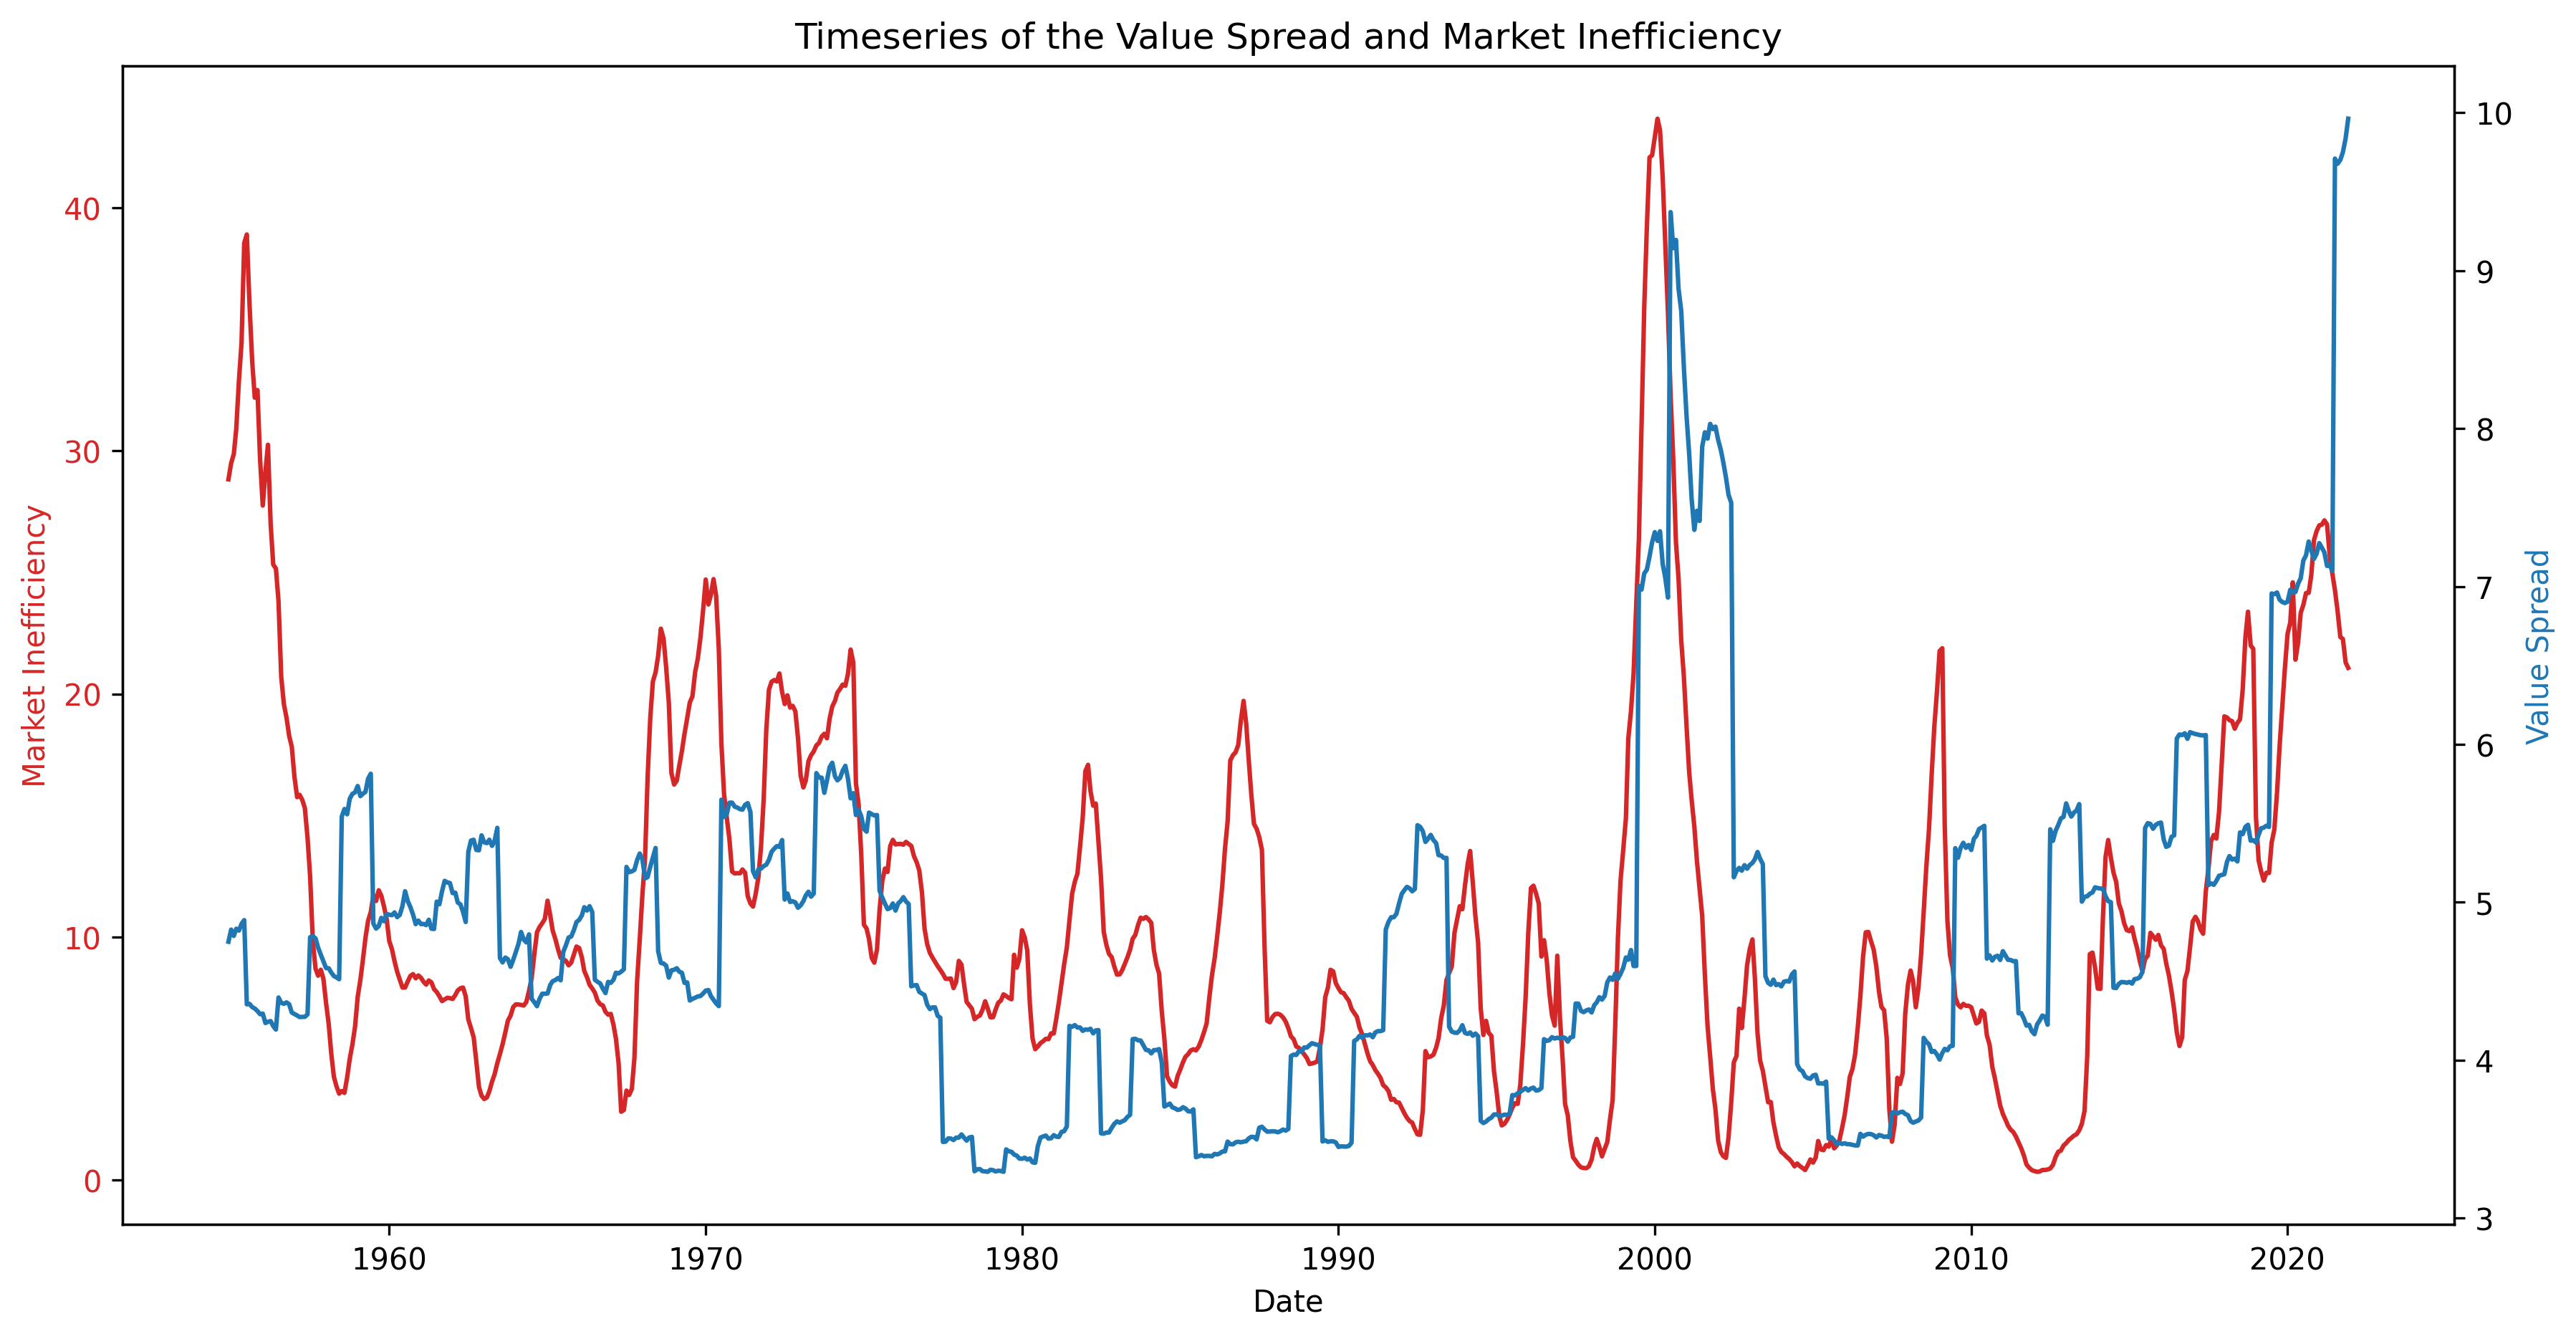
\includegraphics[width=1\textwidth]{../figs/Value_Spread_and_Market_Inefficiency.png}
    \caption{The value spread, and market inefficiency move together, and have been increasing in tandem for the last decade.}
    \label{value_spread_beta_sse}
\end{figure}